\label{chapter:coordinatingstorage}

% re-iterate the introduction
In this dissertation we optimized distributed computing workflows on a campus grid.  We were interested in optimizing a researcher's use of the computational and storage resources on the campus to increase the reliability and decrease the time to solution for scientific results.  We first extended prior work to enhance the computational capabilities of researchers on a campus.  We then expanded our work to the data needs of modern workflows on the campus.

% Conclusion of BOSCO
Bosco is used to effortlessly create a remote submission endpoint on a cluster without requiring the administrator to install any software.  Bosco is a remote submission framework based upon HTCondor.  It uses the SSH protocol to submit and monitor remotely submitted jobs.  Additionally, it performs file transfers using the same SSH connection.

Improving the user experience was a primary goal of Bosco.  We addressed the user experience by improving the interaction with the user during the installation / configuration.  Another problem area we found is when a user must debug issues with distributed software.  In order to address this, we created a traceroute like utility.  The traceroute utility tests every step of the job submission process, from network access to a properly configured remote scheduler.  If an error is found at any step of the traceroute, a useful message is given to the user, including possible steps to fix the problem.

Bosco and the Campus Factory combine to make an easy to use framework that can distribute jobs to many computational clusters on a campus.  Users are able to effectively distribute their processing to multiple clusters using this framework.  I showed that Bosco transparently and effectively distributes computational jobs across multiple clusters on a campus, while maintaining simple usage for users.

Bosco's usage has increased since I originally published the Bosco paper.  For example, it is heavily used by the University of Chicago in order to submit OSG processing to opportunistic resources around the country.  They find Bosco useful since it does not require the installation of any software on the remote cluster.  Additionally, it has been used in several publications by the CMS experiment when they have used opportunistic resources for data processing.

% Conclusion of the CacheD
For data distribution on the campus, we have presented the HTCondor CacheD, a framework to decrease the stage-in time for large shared input datasets.  Our experiments proved that the CacheD decreases stage-in time for these datasets.  Additionally, the transfer method that the CacheD used can significantly affect the stage-in time of the jobs.

The BitTorrent transfer method proved to be a efficient method to transfer caches from the originator to the execution hosts.  In fact, the transfer time for jobs did not increase as the number of distinct nodes requesting the data increased.  Any bottlenecks that surround the cluster are therefore irrelevant using the BitTorrent transfer method.  In addition, we found that the CacheD using BitTorrent transfer method out performed the popular HTTP transfer method on the Open Science Grid.

% Conclusion of the Policy Language
In a distributed computing system, independent agents are designed to act on behalf of entities such as users, hosts, or entire clusters.  A policy language must exist so that the entities can express their goals to the agents.  

I have designed a policy language based on the HTCondor ClassAds that can be used for expressing policy in data distribution.  I have identified three interaction points for caching agents and designed the semantics for their interaction.  The policy language has been implemented in the CacheD, where it has been tested in Chapter \ref{chapter:campusdatadistribution}. 

Through Bosco, I have created a framework for easy-to-use job submission on the campus.  Through the CacheD, I have created an efficient data distribution agent for the campus.  And through a policy language I created, storage agents can negotiate and represent the users and resource owners goals.  This has created a comprehensive picture for campus computing.

\section{Future Work}

\subsection{Debugging}
% Improved debugging for Bosco
Debugging in distributed computing has always been a challenge.  Many different systems working together can create barriers for message and error propagation.

Debugging in Bosco has always been difficult.  To alleviate some of the debugging burden, we created the \texttt{traceroute} utility described in Section \ref{sec:boscotraceroute}.  But that is not enough to solve every issue.  See Figure \ref{fig:boscojobsubmitflowconclusion} for the flow of job submission in Bosco.

\begin{figure}[h!t]
	\centering
	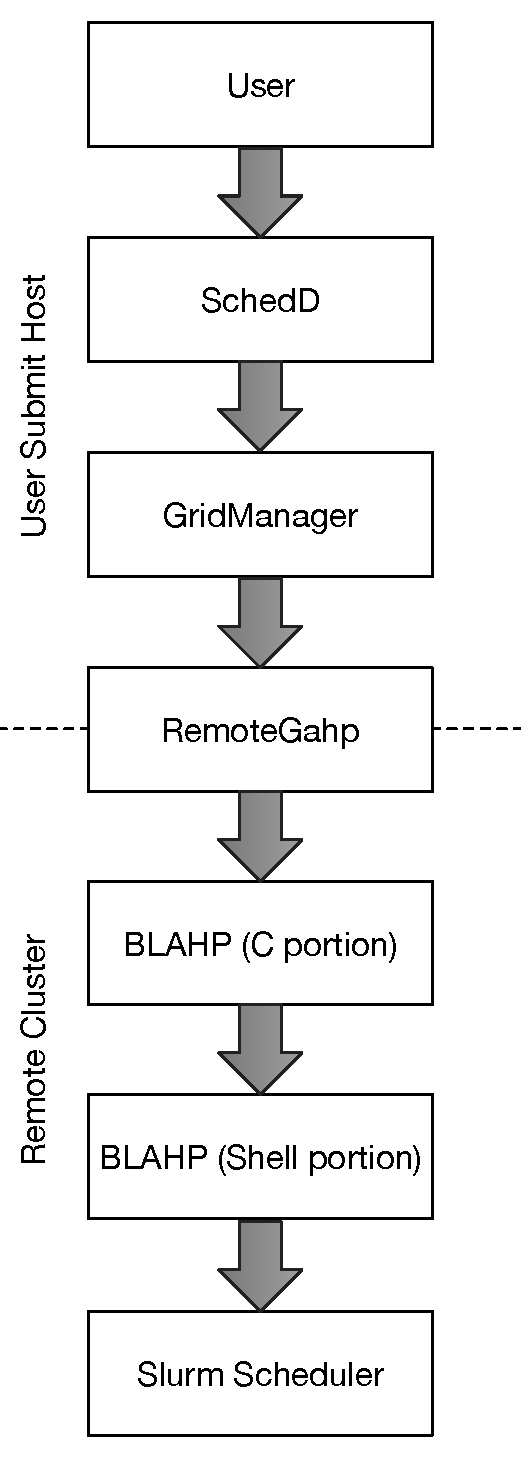
\includegraphics[width=0.3\textwidth]{images/JobSubmitFlow.pdf}
	\caption{Bosco Job Submission Flow From Submission Host to Remote Cluster}
	\label{fig:boscojobsubmitflowconclusion}
\end{figure}

In Figure \ref{fig:boscojobsubmitflowconclusion}, the Bosco job submission starts at the user, and goes through 6 daemons before the submission reaches the Slurm Scheduler on the remote cluster.  An error can occur at each step in this process.  The error propagation must propagate back to the user if there is an error.  But, propagating the error is very difficult, since each daemon has different methods of internal error propagation.  For example, the GridManager can propagate an error back to the SchedD through HTCondor ClassAds.  But, the Blahp's shell portion cannot propagate an error back except through the linux standard error.

Further work need to be done, and parts of the Bosco submission chain need to be modified or refined in order to enable improved error propagation

\subsection{Flexible Transfer Types}
% Addition of transfer types, and flexible system for defining transfer methods

The CacheD currently has support for two transfer methods, the Direct and the BitTorrent methods.  The BitTorrent method uses the libtorrent library directly for transfers.

The Direct method uses HTCondor's file transfer service.  The file transfer service is expandable through file transfer plugins.  The CacheD would benefit from enabling similar file transfer plugins in order to allow proper negotiation of file transfer methods.

A possible solution is to build off of the file transfer plugins method.  An executable advertises it's transfer capabilities to the CacheD, which in turn uses those capabilities to negotiate with other CacheDs for transferring caches.


\subsection{Co-Scheduling of Data and Computation}

% Scheduling jobs with CacheD
Scheduling of jobs with the caching data could optimize job placement.  Currently, there is no knowledge of the cache placement when scheduling a job.  If the scheduler knew where replicas of the cache were located, it could schedule the jobs run where the replicas are located.  Running the job near the cache will eliminate stage-in time.

Currently, the CacheD reports each cache stored locally to the cache's origin. The origin CacheD keeps a data structure of the locations of the cache replicas.

The job needs to specify the caches are required for the job to run.  The scheduler would then call out to the origin CacheD to see if the cache is located at the target node.  This could be done using the HTCondor ClassAd library plugins.


% Not only where the cache is, but with the policy language, we can guess where the job will be.



% optimize black holes for bittorrent


